\documentclass{beamer}
% use this instead for 16:9 aspect ratio:
%\documentclass[aspectratio=169]{beamer}
\usepackage{etex}
\usepackage{verbatim}
\reserveinserts{28}
\usetheme{ETHbeamer}

\colorlet{ETHcolor1}{ETHc}
\colorlet{ETHcolor2}{ETHc}

\author{Benjamin Ellenberger}
\institute{INI:  Institute of Neuroinformatics}

\title{Emergent gait periodicity in artificially evolved creatures on unknown terrains}

\date{2015-05-13}

%%TODO: Add todo feature
%%TODO: Optimize with presentation tips

% uncomment if you do not want to use a department logo
%\deplogofalse


\begin{document}

\titleframe

\section{Are we alone in the universe?}

%\begin{frame}

%  \frametitle{Contents}
%  \tableofcontents[currentsection]
%\end{frame}

% Are we alone in the universe?
\begin{minimalframe}
	\hspace*{-1.1cm}
	\vspace*{1cm}
	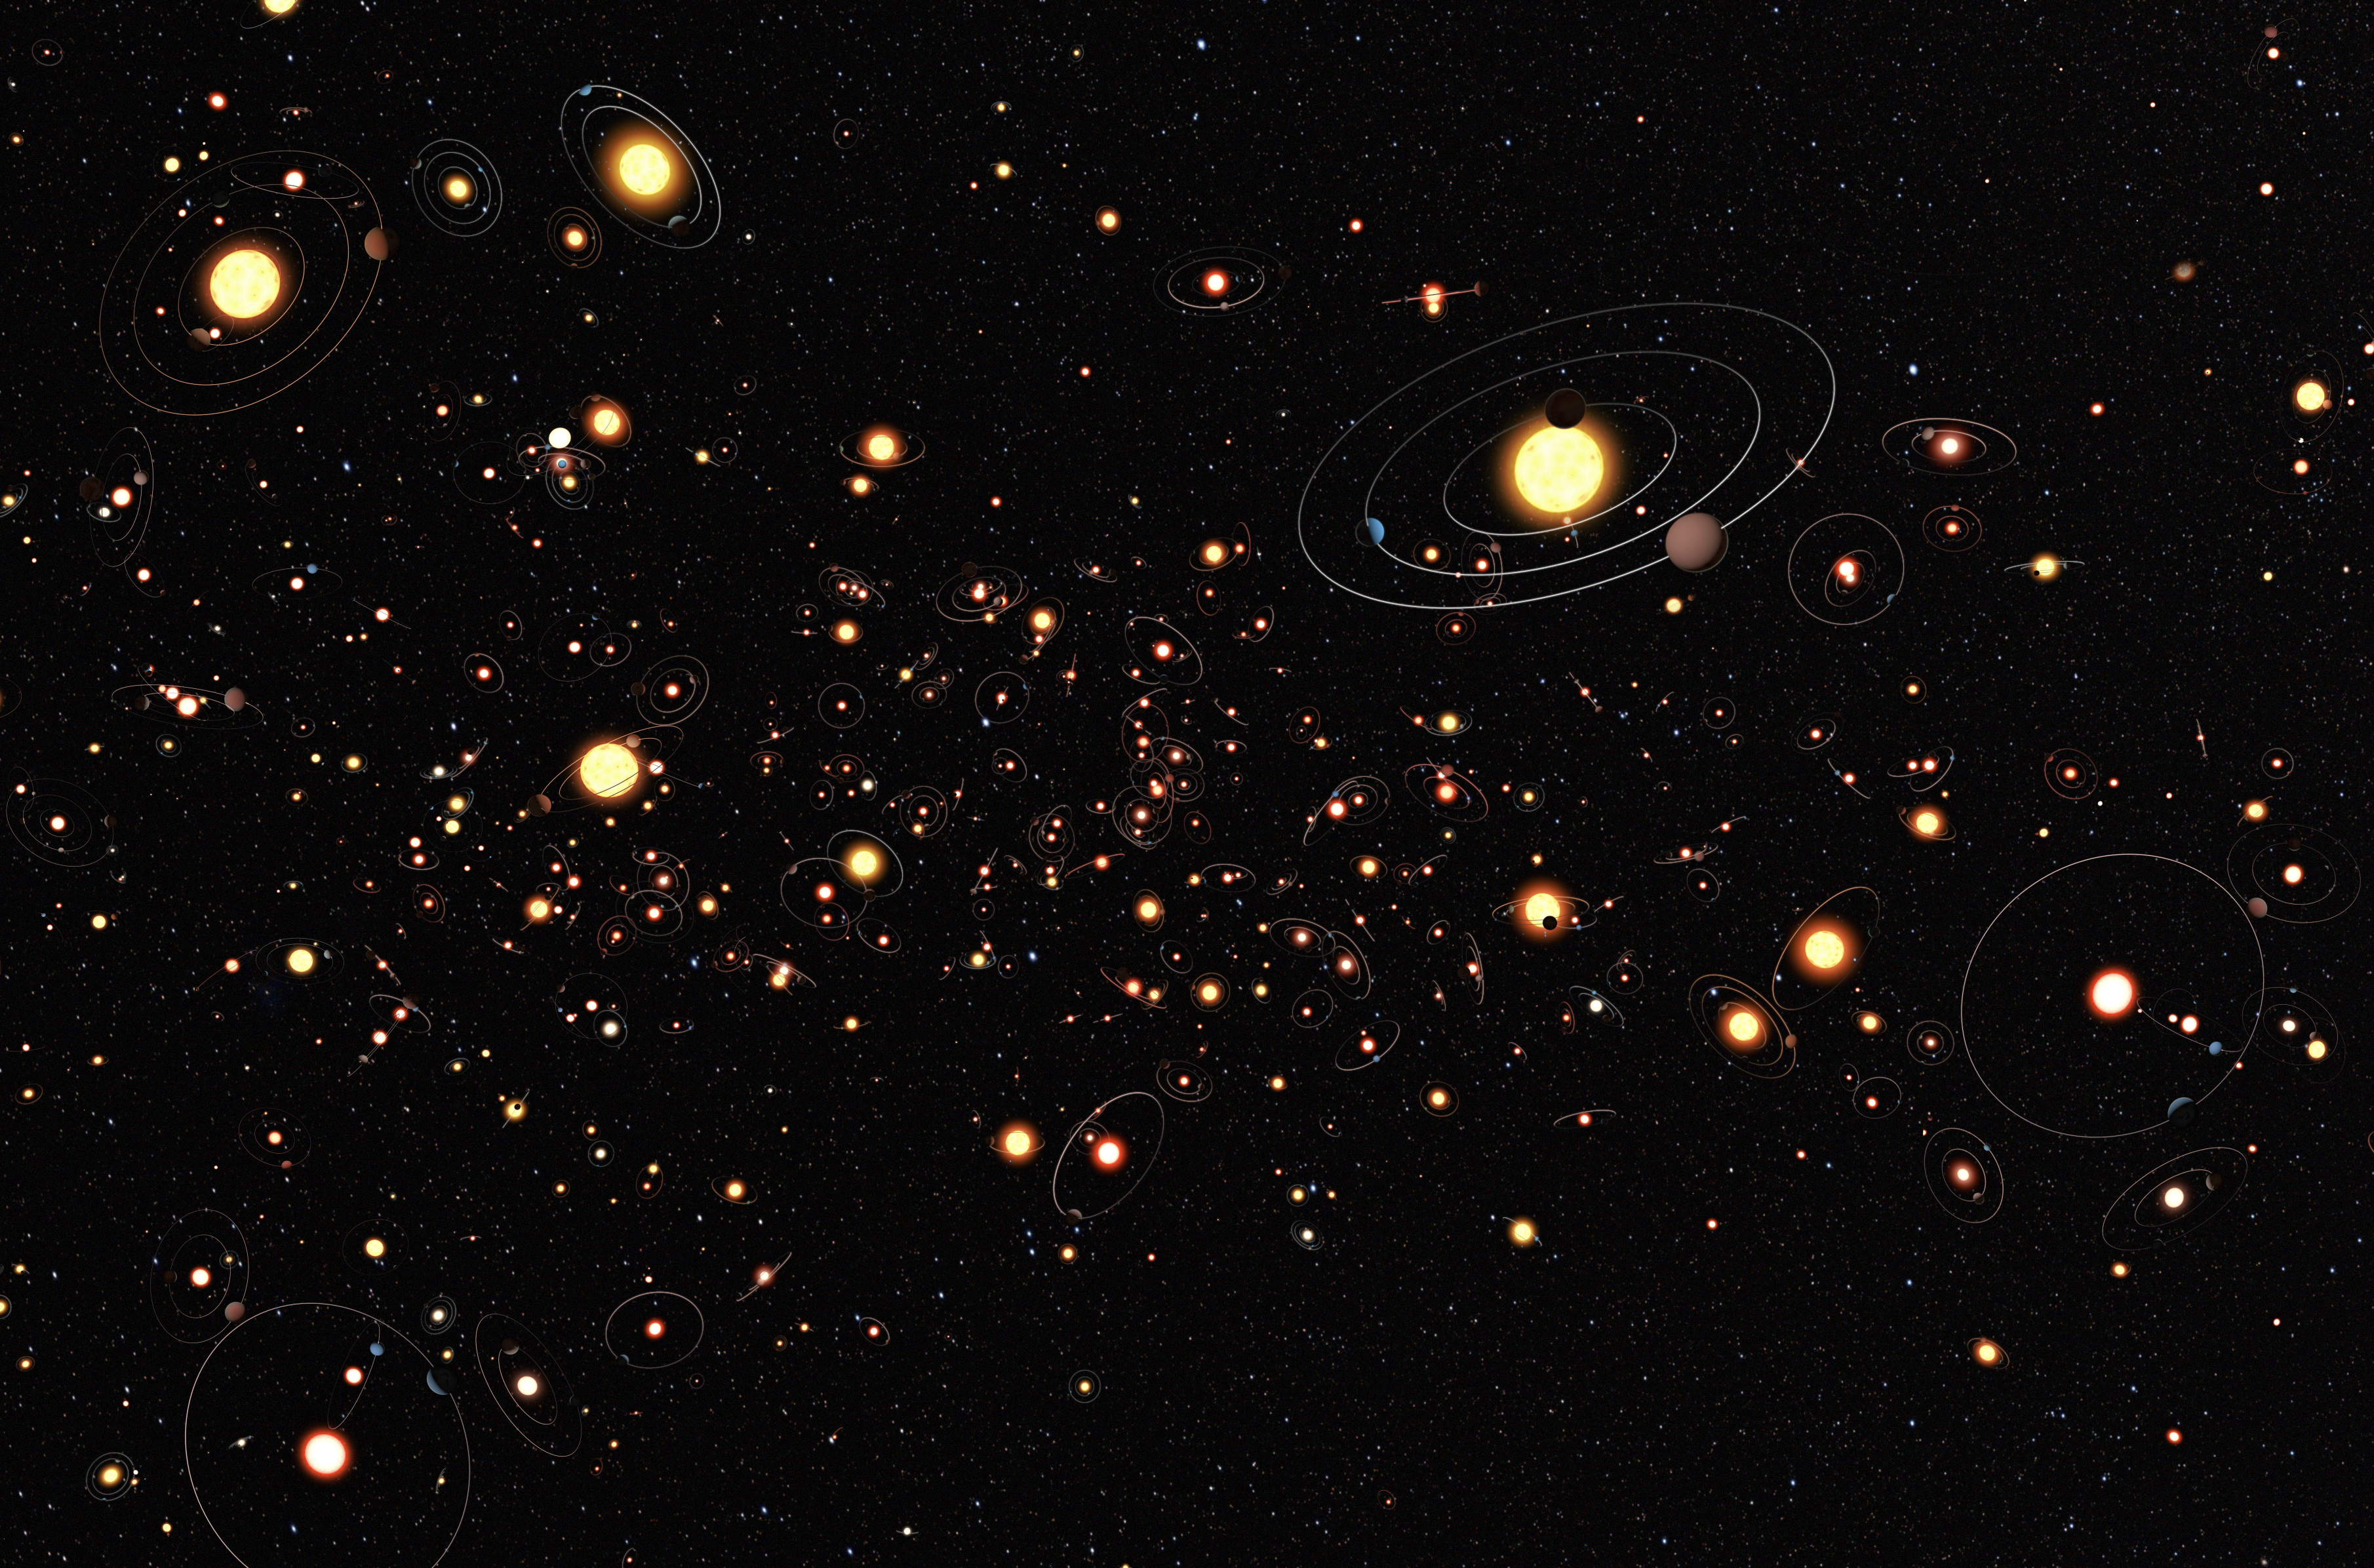
\includegraphics[width=1.4\textwidth,clip]{figs/Planets_everywhere.jpg}
	
\end{minimalframe}

% Life as it is vs. life as it could be
\begin{frame}

	\frametitle{Life as it is vs. life as it could be}
	\begin{center}
	\includegraphics[width=0.8\textwidth,clip]{figs/tree_of_life_cut.png}\\\vspace{1em}
	\includegraphics[width=0.75\textwidth,clip]{figs/art_tree_of_life_cut.png}
	\end{center}

\end{frame}

\begin{frame}

		  \begin{columns}
   \column{0.5\textwidth}
   
   \frametitle{Goals}
	\begin{itemize}
 	 \visible<1->{
	\item Build robots that are not only capable but also more adaptive (Engineering goal)
	 }
	 \visible<2>{
	\item Structures and strategies that always tend to evolve (Academic goal)
	}
	\end{itemize}
     \visible<1->{
     \column{0.5\textwidth}
      \includegraphics[width=2in, clip] {figs/goals.jpg}
      }
  \end{columns}
\end{frame}

\section{Simple limiters theory}

\begin{frame}

  \frametitle{Contents}
  \tableofcontents[currentsection]
\end{frame}

% Simple limiter theory
\begin{frame}
	\frametitle{Simple limiters}
	  \begin{columns}
   \column{0.5\textwidth}
 \begin{itemize}
 	 \visible<1->{
	    \item Generally the chaos controller is more complex than the system it controls
	 }
	 \visible<2>{
    		\item Not true for the simple limiter
    	}

    	\visible<1->{
    	\vspace*{2.9em}
    	\includegraphics[width=1.9in, clip] {figs/chaotic-driven-pendulum-pcmap.jpeg}
    	}
     \end{itemize}
     \visible<1->{
     \column{0.5\textwidth}
      \includegraphics[width=1.5in, clip] {figs/chaotic-driven-pendulum.png}\\
      \includegraphics[width=1.65in, clip] {figs/chaotic-driven-pendulum-bifurcationmap.jpeg}
      }
  \end{columns}
\end{frame}

%% Types of simple limiters in nature
\begin{frame}
	\frametitle{Simple limiters in nature}
	\begin{columns}
	\column{.6\textwidth}
	\begin{itemize}
	\visible<2->{
	\item Muscle length \& joint limits
	}
	
	\visible<3->{
	\item The weight of the limbs
	}
	
	\visible<4->{
	\item The relative position of limbs connected by joints\\ (Direction of force applied to joints)
	}
	
	\visible<5>{
	\item The fact that physical objects can not interpenetrate each other
	}
	
	\end{itemize}
\column{.45\textwidth}
     \visible<1->{
		%http://jonbarron.org/article/physiology-muscles
	\includegraphics[width=1\textwidth]{figs/natural-limiter-arm-muscle.jpg}
	}
  \end{columns}
\end{frame}

\begin{frame}
\frametitle{Simple limiters cont.}

%%TODO: Add videolinks for their walks
\href{run:figs/videos/normal-dude.mp4}{\includegraphics[width=0.19\textwidth]{figs/limiters/1.png}}
\href{run:figs/videos/tiny-dude.mp4}{\includegraphics[width=0.19\textwidth]{figs/limiters/2.png}} 
\href{run:figs/videos/tall-dude.mp4}{\includegraphics[width=0.19\textwidth]{figs/limiters/3.png}} 
\href{run:figs/videos/super-wide-dude.mp4}{\includegraphics[width=0.19\textwidth]{figs/limiters/4.png}} 
\href{run:figs/videos/super-neck-dude.mp4}{\includegraphics[width=0.19\textwidth]{figs/limiters/5.png}} 
\tiny{Source: Geijtenbeek et al. (Vol. 32, Nr. 6 SIGGRAPH 2013)}
\end{frame}

%% Will simple limiters be used if they do not need to be used
\begin{frame}
	\frametitle{In silico\footnote{In silico = in simulation}: Will the simple limiters be used?}
	\begin{columns}
	\column{0.6\textwidth}
	\begin{itemize}
	\visible<2->{
	\item Hypothesis 1: Simple limiters are an omnipresent feature used to reduce the control complexity and to control chaotic movement
	}
	\visible<3->{
	\item Hypothesis 2: If the world is flat then less simple limiters are used, if the world is dynamic and bumpy then more simple limiters are used.
	}
	\visible<4->{
	\item Question remains: Can you live limitless?
	}
	\end{itemize}
	\column{0.5\textwidth}
	\visible<1->{
	\includegraphics[width=0.8\textwidth]{figs/Sims.png}\\
	\includegraphics[width=0.8\textwidth]{figs/MarsMadness.png}
	}
	\end{columns}
\end{frame}


\section{Methods}

\frame{

  \frametitle{Contents}
    \tableofcontents[currentsection]
}
\note{}

\subsection{Evolution}

\frame{

  \frametitle{Evolving Virtual Creatures}
  
  \begin{columns}
   \column{0.5\textwidth}
 \begin{itemize}
  	\visible<2->{
	     \item Creatures are built from 3D Primitives and Joints
	}
	
	\visible<3->{
    	\item Sensors, Controller and Effectors make it move
    	}
    	
 	\visible<4->{
    	\item Body and controller co-evolved
 	}
     \end{itemize}
     
     \column{0.5\textwidth}
      \visible<1->{
      \includegraphics[width=2in, clip] {figs/creatures.jpg} 
      }
  \end{columns}
  }
\note{}

\subsection{Genetic language}
\frame{

  \frametitle{Genetic language: Genotype}

\begin{tikzpicture}
   \foreach \c/\i/\t [count=\n] in  
        {blue!20/RootLimb/2,green!20/Limb1/1,orange!20/Limb2/0.8,red!20/Limb3/0.5} 
           \node[draw,fill=\c,minimum height=\t * 1.5cm,minimum width = \t * 1cm,xshift=\n* 2cm](N\n){\i} ;
\draw[dashed,->,line width=0.5mm] (N1.south) to [out=-50,in=-150] node[below] {Branch/2} (N2.south);
\draw[dashed,->,line width=0.5mm] (N2.north) to [out=50,in=150] node[above] {Branch/2} (N3.north);
\draw[dashed,->,line width=0.5mm] (N2.south) to [out=-50,in=-150] node[below] {Branch/2} (N4.south);

\end{tikzpicture}

  \begin{itemize}
\item \textbf{Limb} Part of creature body
\end{itemize}

  
  }
\note{}

\frame{
 \frametitle{Genetic language: Phenotype}

% Set the overall layout of the tree
\tikzstyle{level 1}=[level distance=1cm, sibling distance=6cm]
\tikzstyle{level 2}=[level distance=1.5cm, sibling distance=1.4cm]

% Define styles
\tikzstyle{rl}=[draw,fill=blue!20,minimum height=3cm,minimum width=2cm]
\tikzstyle{l1}=[draw,fill=green!20,minimum height=1.5cm,minimum width=1cm]
\tikzstyle{l2}=[draw,fill=orange!20,minimum height=1.2cm,minimum width=0.8cm]
\tikzstyle{l3}=[draw,fill=red!20,minimum height=0.75cm,minimum width=0.5cm]

\begin{tikzpicture}[grow=down, sloped]
\node[rl] {RootLimb}
    child {
            node[l1] {Limb1}
            child {
                node[l2] {Limb2}
            }
            child {
                node[l3] {Limb3}
            }    
            child {
                node[l3] {Limb3}
            }
            child {
                node[l2] {Limb2}
            }
    }
    child {
            node[l1] {Limb1}
            child {
                node[l2] {Limb2}
            }
            child {
                node[l3] {Limb3}
            }    
            child {
                node[l3] {Limb3}
            }
            child {
                node[l2] {Limb2}
            }
    };
\end{tikzpicture}
  }
\note{}

\frame{

  \frametitle{Genetic language: Phenotype cont.}
  \begin{center}
\includegraphics[width=0.8\textwidth, clip] {figs/Sims_Evolve.png}
  \end{center}
  }
\note{}

\frame{

  \frametitle{Execution of creatures}
  \begin{columns}
  \column{0.45\textwidth}
\includegraphics[width=1\textwidth, clip] {figs/brain-body-cycle.png}
 \column{0.55\textwidth}
\includegraphics[width=1\textwidth, clip] {figs/execution.png}
  \end{columns}
  }
\note{}

\subsection{Fitness evaluation}
\frame{

  \frametitle{Fitness evaluation}

\begin{itemize}
\item Fitness evaluation framework
\item A creature is simulated for a certain evaluation time during which the fitness function measures the fitness of the creature
\item Could evaluate multiple fitness functions at the same time
\end{itemize}

  
  }
\note{}

\frame{

  \frametitle{Velocity as the fitness function}

\begin{itemize}
\item Sampling of position over time and average over all limbs
\item Moved distance in a certain time interval
\item Continuous average
\item Expectations: Some really moving creatures and some finding an exploit to the fitness function
\end{itemize}
  
  }
\note{}

\subsection{Evolution}
\frame{

  \frametitle{Evolution}

\begin{itemize}
\item Selection: Only a certain percentage of creatures are selected for new generation
\item Cross-over: Only certain percentage of creatures are allowed to breed
\item Mutation
\begin{itemize}
\item Other creatures are subject to mutation
\item Mutation of gene
\item Mutation of gene attributes
\item Mutation of gene branches
\end{itemize}
\item Successful creatures stay in the population and the population is refilled with newly bred and mutated ones
\end{itemize}
  
  }
\note{}

\subsection{Controller}
\frame{

  \frametitle{Controller}
  \begin{columns}
  \column{0.5\textwidth}
  \begin{itemize}
  \item Sine-wave controller taking frequency, amplitude, X-shift,Y-shift as input which are determined evolutionarily.
  \end{itemize}
  \column{0.5\textwidth}
  \includegraphics[width=2in, clip] {figs/osc-symbol.png}
  \end{columns}
}
\note{}

\subsection{Why Periodicity?}
\frame{

  \frametitle{Why Periodicity?}

\begin{center}
  \href{run:figs/videos/dynamic-gait.mp4}{\includegraphics[width=0.8\textwidth, clip] {figs/dynamic-gait.png}}
  \end{center}

}
\note{}

\section{Meet \& Greet with the Creatures}

\frame{

  \frametitle{Contents}
    \tableofcontents[currentsection]
}
\note{}

\frame{

  \frametitle{Creatures}
  \begin{figure}[tp]
    \centering
    \includegraphics[width=3in, clip] {figs/creatures/Minemonics-05112015_184631057.jpg}
\end{figure}
  }
\note{}

\frame{

  \frametitle{Creatures}
  \begin{figure}[tp]
    \centering
    \includegraphics[width=3in, clip] {figs/creatures/Minemonics-05112015_190654362.jpg}
\end{figure}
  }
\note{}


\frame{

  \frametitle{Creatures}
  \begin{figure}[tp]
    \centering
    \includegraphics[width=3in, clip] {figs/creatures/Minemonics-05112015_190853660.jpg}
\end{figure}
  }
\note{}

\frame{

  \frametitle{Creatures}
  \begin{figure}[tp]
    \centering
    \includegraphics[width=3in, clip] {figs/creatures/Minemonics-05112015_190947481.jpg}
    \caption{Simulate 50 creatures at the same time}
\end{figure}
  }
\note{}

\frame{

  \frametitle{Creatures}
  \begin{figure}[tp]
    \centering
    \includegraphics[width=3in, clip] {figs/creatures/Minemonics-05112015_191706383.jpg}
    \caption{Simulate 1000 creatures at the same time}
\end{figure}
  }
\note{}

\frame{

  \frametitle{Creatures}
  \begin{figure}[tp]
    \centering
     \href{run:figs/videos/Movement.mp4}{\includegraphics[width=0.7\textwidth, clip] {figs/kerfuffle.png}}
    \caption{Short video}
\end{figure}
  }
\note{}



\section{Outlook}

\frame{

  \frametitle{Contents}
    \tableofcontents[currentsection]
}
\note{}

\subsection{Extensions: Evolutionary Algorithm}
\frame{

  \frametitle{Extensions: Evolutionary Algorithm}
  
  \begin{itemize}
  \item Different types of evolutionary selection and evaluation
  \item The system does not use any parallelization
  \item The phenotype could be more natural
  \item Sensor and actuator types
  \item More logging for data analysis (different live-views)
  \end{itemize}
}
\note{}

\subsection{Extensions: Controllers}
\frame{

  \frametitle{Extensions: Controllers}
  \begin{columns}
  \column{0.5\textwidth}
  \begin{itemize}
  \item Different types of controllers taking sensors as inputs
  \item Deep Neural Networks especially the LSTM neural network
  \item Other ideas I have until then
  \end{itemize}
  \column{0.5\textwidth}
  \includegraphics[width=1.5in, clip] {figs/NN.png} 
  \end{columns}
}
\note{}

\subsection{Other settings}
\frame{

  \frametitle{Other settings}
  \begin{itemize}
  \item Island genetic algorithm (Possible via planets)
  \item Competitions of individuals
  \item Implicit fitness functions (survival of the fittest in a virtual world)
  \item Information theoretic measures such as the transfer entropy for neural networks
  \end{itemize}
  
}
\note{}

\begin{frame}

\newcommand{\quadrat}{(0,0mm)--(0mm,5mm)--(5mm,5mm)--(5mm,0mm)--(0mm,0mm);}
\begin{center}
	\hspace{-8mm}
	\begin{tikzpicture}[overlay]
		{\draw[ETHa,fill=ETHa] \quadrat}\label{ETH1}
	\end{tikzpicture}
	\hspace{10mm}
	\begin{tikzpicture}[overlay]
		{\draw[ETHb,fill=ETHb]\quadrat}\label{ETH2}
	\end{tikzpicture}
	\hspace{10mm}
	\begin{tikzpicture}[overlay]
		{\draw[ETHc,fill=ETHc]\quadrat}\label{ETH3}
	\end{tikzpicture}
	\hspace{10mm}
	\begin{tikzpicture}[overlay]
		{\draw[ETHd,fill=ETHd] \quadrat}\label{ETH4}
	\end{tikzpicture}
	\hspace{10mm}
	\begin{tikzpicture}[overlay]
		{\draw[ETHe,fill=ETHe] \quadrat}\label{ETH5}
	\end{tikzpicture}
	\hspace{10mm}
	\begin{tikzpicture}[overlay]
		{\draw[ETHf,fill=ETHf] \quadrat}\label{ETH6}
	\end{tikzpicture}
	\hspace{10mm}
	\begin{tikzpicture}[overlay]
		{\draw[ETHg,fill=ETHg] \quadrat}\label{ETH7}
	\end{tikzpicture}
	\hspace{10mm}
	\begin{tikzpicture}[overlay]
		{\draw[ETHh,fill=ETHh] \quadrat}\label{ETH8}
	\end{tikzpicture}
	\hspace{10mm}
	\begin{tikzpicture}[overlay]
		{\draw[ETHi,fill=ETHi] \quadrat}\label{ETH9}
	\end{tikzpicture}
\end{center}
\vspace*{3em}
\begin{itemize}
\item Any questions?
\item What experiments would you have in mind?
\item What else would you change, extend, enhance, improve etc.?
\item If you have any ideas later, email me: be.ellenberger@gmail.com
\item You can look at my progress: https://github.com/benelot/minemonics
\end{itemize}

\end{frame}


\frame{

  \frametitle{References}
  \begin{itemize}
  \item Sims K. - Evolving Virtual Creatures (1994)
  \item Sims K. - Evolving 3D Morphology and Behavior by Competition (1994)
  \item Krcah P. - Evolving Virtual Creatures Revisited (2007)
  \item Corron N. et al. - Controlling Chaos with Simple Limiters (2000)
  \item Schmidt N. - Bootstrapping perception using information theory: case studies in a quadruped running robot running on different grounds (2013)
  \item Geijtenbeek T. - Flexible Muscle-Based Locomotion for Bipedal Creatures (2013)
  \item Stoop R. - Theory and Simulation of Neural Networks (2014)
  \end{itemize}
}
\note{}

\begin{comment}

% Example slides
\begin{frame}
\textbf{Some mathematical specialities}

\ETHbox{0.8\textwidth}{% define the ETHbox
  \begin{theorem}[Murphy (1949)]\label{murphy}
    Anything that can go wrong, will go wrong.
  \end{theorem}
}

\begin{proof}
  A special case of Theorem \ref{murphy} is proven in %\citet{matthews1995}.
\end{proof}
\end{frame}

\begin{titlestyleframe}
\frametitle{Title Page}

\color{white} The title page is created using the \texttt{\textbackslash titleframe} command.

The title page background can also be used on other frames (or for a customised title frame) using the \texttt{titlestyleframe} environment.
\end{titlestyleframe}

\begin{frame}
\frametitle{Normal Frame}
The normal frame looks like this. It is created using the \texttt{frame} environment.
\end{frame}
\begin{inverseframe}
  \frametitle{Inverse Slides}
  %\color{white}
The inverted frame looks like this. It is created using the \texttt{inverseframe} environment.

 
\end{inverseframe}

\begin{minimalframe}
  \frametitle{Minimal Frame}
The minimal frame looks like this. It is created using the \texttt{minimalframe} environment.
  
\end{minimalframe}

\end{comment}

\end{document}
